% !TeX program = xelatex
\documentclass[
  convert={density=500, size=600, outext=.png},
  border=2pt
]{standalone}

\usepackage{fontspec}
\defaultfontfeatures{Ligatures={NoCommon,%
			NoDiscretionary,%
			NoHistoric,%
			NoRequired,%
			NoContextual}}
\setsansfont{Carlito}[%
	SmallCapsFeatures={Letters=SmallCaps},%
	SmallCapsFont={Roboto},%
	ItalicFeatures={SmallCapsFont=Roboto-Italic},%
	BoldFeatures={SmallCapsFont=Roboto-Bold},%
	BoldItalicFeatures={SmallCapsFont=Roboto-BoldItalic}%
]

\usepackage{tikz}
\usepackage{tikz-cd}
\usetikzlibrary{%
	calc,%
	arrows.meta,%
	arrows,%
	automata,%
	overlay-beamer-styles,%
	snakes,%
	shapes.arrows,%
	shapes.geometric,%
	shapes.symbols,%
	fit,%
	positioning,%
	decorations.pathreplacing,%
	backgrounds,%
}
\tikzset{
	>=Triangle,%
	nodes={align=center},%
	comp/.style={%
			draw,%
			rectangle,%
			very thick,%
			rounded corners,%
			minimum width=2.5cm,%
			minimum height=1cm,%
			fill=white},%
	input/.style={draw,%
			rectangle,%
			thick,%
			minimum width=2.5cm,%
			minimum height=1cm,%
			fill=white},%
	classnode/.style={%
			fill=cgreenlight,%
			rectangle,%
			draw,%
			inner xsep=0},%
	interfacenode/.style={%
			fill=corangelight,%
			rectangle,%
			draw,%
			inner xsep=0},%
	abstractclassnode/.style={%
			fill=cbluelight,%
			rectangle,%
			draw,%
			inner xsep=0},%
	inlinenode/.style={%
			inner xsep=.5cm,%
			minimum height=.6cm},%
}

\definecolor{reddy}{RGB}{172, 0, 51}
\definecolor{dkred}{rgb}{.6, 0, 0}
\definecolor{dkgreen}{rgb}{0, .5, 0}
\definecolor{dkblue}{rgb}{0, 0, .5}
\definecolor{cred}{RGB}{219, 68, 55}
\definecolor{credlight}{RGB}{250, 227, 225}
\definecolor{cgreen}{RGB}{3, 148, 77}
\definecolor{cgreenlight}{RGB}{209, 251, 230}
\definecolor{cblue}{RGB}{2, 119, 189}
\definecolor{cbluelight}{RGB}{208, 237, 254}
\definecolor{corange}{RGB}{173, 128, 2}
\definecolor{corangelight}{RGB}{253, 219, 123}
\newcommand{\cblue}[1]{\textcolor{cblue}{#1}}
\newcommand{\bfcblue}[1]{\textcolor{cblue}{\textbf{#1}}}
\newcommand{\cred}[1]{\textcolor{cred}{#1}}
\newcommand{\bfcred}[1]{\textcolor{cred}{\textbf{#1}}}
\newcommand{\cgreen}[1]{\textcolor{cgreen}{#1}}
\newcommand{\bfcgreen}[1]{\textcolor{cgreen}{\textbf{#1}}}
\newcommand{\corange}[1]{\textcolor{corange}{#1}}
\newcommand{\bfcorange}[1]{\textcolor{corange}{\textbf{#1}}}
\newcommand{\interfacename}[1]{\underline{\textbf{\textit{#1}}}}
\newcommand{\absclassname}[1]{\textbf{\textit{#1}}}
\newcommand{\classname}[1]{\textbf{#1}}

\usepackage{amsmath}
\usepackage{amsfonts}
\usepackage{amssymb}

\usepackage{silence}
\WarningsOff*


\begin{document}
\sffamily

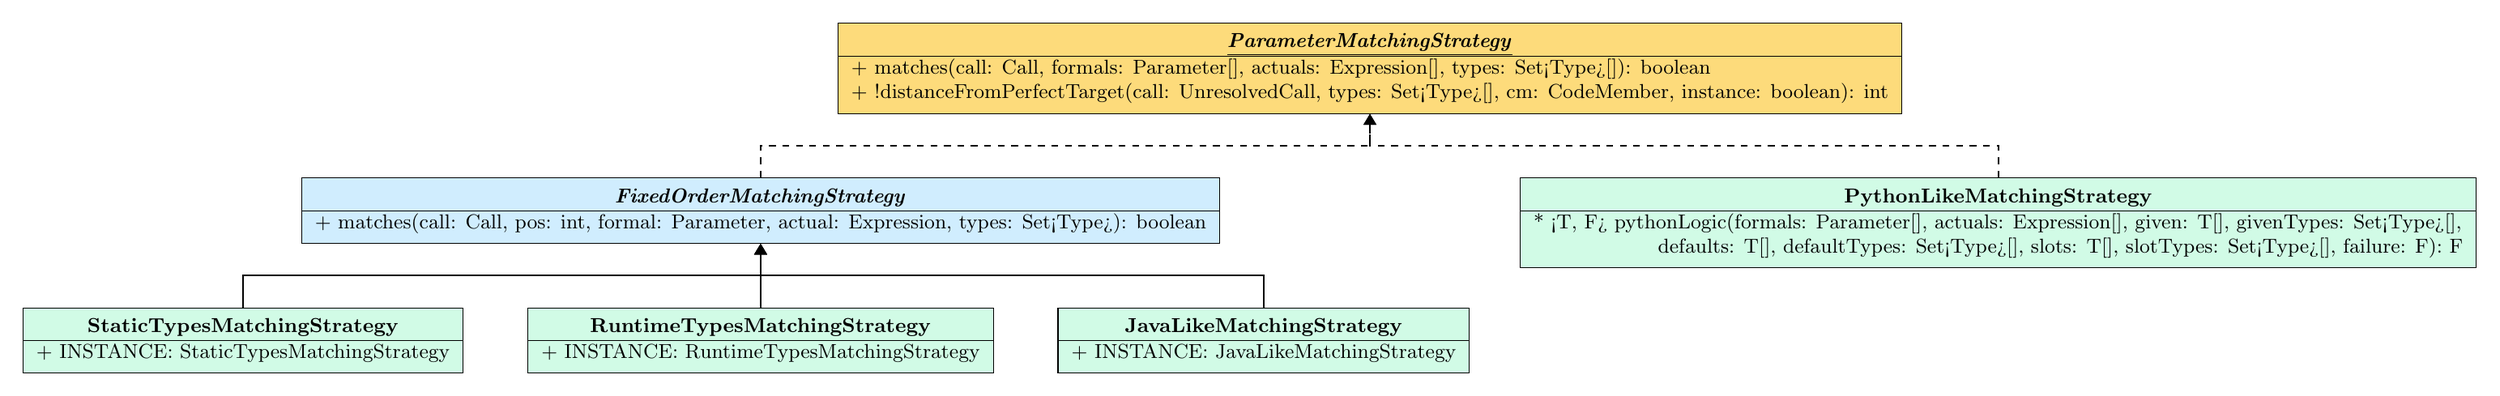
\begin{tikzpicture}[nodes={font={\small}, minimum width=3.5cm}]%
	\node[interfacenode] (pms) {\begin{tabular}{l}
			\multicolumn{1}{c}{\interfacename{ParameterMatchingStrategy}}                                                  \\
			\hline
			+ matches(call: Call, formals: Parameter[], actuals: Expression[], types: Set<Type>[]): boolean                \\
			+ !distanceFromPerfectTarget(call: UnresolvedCall, types: Set<Type>[], cm: CodeMember, instance: boolean): int \\
		\end{tabular}};

	\node[classnode] (plm) [below right=1cm and -6cm of pms] {\begin{tabular}{l}
			\multicolumn{1}{c}{\classname{PythonLikeMatchingStrategy}}                                                       \\
			\hline
			* <T, F> pythonLogic(formals: Parameter[], actuals: Expression[], given: T[], givenTypes: Set<Type>[],           \\
			$\qquad\qquad\qquad$defaults: T[], defaultTypes: Set<Type>[], slots: T[], slotTypes: Set<Type>[], failure: F): F \\
		\end{tabular}};

	\node[abstractclassnode] (foms) [below left=1cm and -6cm of pms] {\begin{tabular}{l}
			\multicolumn{1}{c}{\absclassname{FixedOrderMatchingStrategy}}                                     \\
			\hline
			+ matches(call: Call, pos: int, formal: Parameter, actual: Expression, types: Set<Type>): boolean \\
		\end{tabular}};

	\node[classnode] (rts) [below=of foms] {\begin{tabular}{l}
			\multicolumn{1}{c}{\classname{RuntimeTypesMatchingStrategy}} \\
			\hline
			+ INSTANCE: RuntimeTypesMatchingStrategy                     \\
		\end{tabular}};

	\node[classnode] (sts) [left=of rts] {\begin{tabular}{l}
			\multicolumn{1}{c}{\classname{StaticTypesMatchingStrategy}} \\
			\hline
			+ INSTANCE: StaticTypesMatchingStrategy                     \\
		\end{tabular}};

	\node[classnode] (jlm) [right=of rts] {\begin{tabular}{l}
			\multicolumn{1}{c}{\classname{JavaLikeMatchingStrategy}} \\
			\hline
			+ INSTANCE: JavaLikeMatchingStrategy                     \\
		\end{tabular}};

	\draw[->, thick, dashed] (foms) |- ($(pms.south)+(0,-0.5)$) to (pms);
	\draw[->, thick, dashed] (plm) |- ($(pms.south)+(0,-0.5)$) to (pms);
	\draw[->, thick] (rts) |- ($(foms.south)+(0,-0.5)$) to (foms);
	\draw[->, thick] (sts) |- ($(foms.south)+(0,-0.5)$) to (foms);
	\draw[->, thick] (jlm) |- ($(foms.south)+(0,-0.5)$) to (foms);
\end{tikzpicture}

\end{document}
